% ============================================================
%  CASTER-ZT — Research Presentation  (20 minutes)
%  Style: clean academic Beamer, state-of-the-art
% ============================================================
\documentclass[aspectratio=169,10pt]{beamer}

% ---------- Theme & Colours ----------
\usetheme{default}
\usecolortheme{default}

\definecolor{navyblue}{RGB}{18,52,104}      % primary deep navy
\definecolor{tealgreen}{RGB}{0,128,115}     % accent teal
\definecolor{lightteal}{RGB}{220,240,238}   % background tint
\definecolor{alertorange}{RGB}{200,80,0}    % alert / highlight
\definecolor{lightgray}{RGB}{245,245,247}   % frame background
\definecolor{midgray}{RGB}{120,120,130}     % secondary text
\definecolor{white}{RGB}{255,255,255}

% Override beamer palette
\setbeamercolor{palette primary}{bg=navyblue,fg=white}
\setbeamercolor{palette secondary}{bg=navyblue!80,fg=white}
\setbeamercolor{palette tertiary}{bg=navyblue!60,fg=white}
\setbeamercolor{structure}{fg=navyblue}
\setbeamercolor{frametitle}{bg=navyblue,fg=white}
\setbeamercolor{title}{fg=white}
\setbeamercolor{subtitle}{fg=white!85}
\setbeamercolor{author}{fg=white!90}
\setbeamercolor{date}{fg=white!80}
\setbeamercolor{institute}{fg=white!85}
\setbeamercolor{block title}{bg=navyblue!12,fg=navyblue}
\setbeamercolor{block body}{bg=lightgray,fg=black}
\setbeamercolor{block title alerted}{bg=alertorange!15,fg=alertorange}
\setbeamercolor{block body alerted}{bg=alertorange!5,fg=black}
\setbeamercolor{block title example}{bg=tealgreen!12,fg=tealgreen!80!black}
\setbeamercolor{block body example}{bg=tealgreen!5,fg=black}
\setbeamercolor{itemize item}{fg=tealgreen}
\setbeamercolor{itemize subitem}{fg=navyblue}
\setbeamercolor{enumerate item}{fg=navyblue}
\setbeamercolor{footline}{fg=midgray,bg=lightgray}
\setbeamercolor{headline}{bg=navyblue}

% ---------- Fonts ----------
\usepackage{lmodern}
\usepackage[T1]{fontenc}
\usepackage[utf8]{inputenc}
\setbeamerfont{title}{size=\large,series=\bfseries}
\setbeamerfont{subtitle}{size=\normalsize,series=\normalfont}
\setbeamerfont{frametitle}{size=\large,series=\bfseries}
\setbeamerfont{block title}{size=\normalsize,series=\bfseries}
\setbeamerfont{footline}{size=\tiny}

% ---------- Frame title ----------
\setbeamertemplate{frametitle}{%
  \nointerlineskip%
  \begin{beamercolorbox}[wd=\paperwidth,ht=0.72cm,dp=0.18cm,leftskip=0.5cm]{frametitle}%
    \usebeamerfont{frametitle}\insertframetitle%
    \ifx\insertframesubtitle\@empty\else%
      \hspace{0.5em}{\footnotesize\color{white!75}|\hspace{0.4em}\insertframesubtitle}%
    \fi%
  \end{beamercolorbox}%
}

% ---------- Footline ----------
\setbeamertemplate{footline}{%
  \begin{beamercolorbox}[wd=\paperwidth,ht=0.4cm,dp=0.15cm]{footline}%
    \hspace{0.4cm}%
    \textcolor{midgray}{CASTER-ZT \textbullet\ G.P.\ Djimefo Kapen, R.\ Al Mallah, S.\ Pierre \textbullet\ Polytechnique Montréal}%
    \hfill%
    \textcolor{navyblue}{\insertframenumber\,/\,\inserttotalframenumber}%
    \hspace{0.4cm}%
  \end{beamercolorbox}%
}

% ---------- No navigation symbols ----------
\setbeamertemplate{navigation symbols}{}

% ---------- Numbered bibliography items ----------
\setbeamertemplate{bibliography item}{\insertbiblabel}

% ---------- Itemize bullets ----------
\setbeamertemplate{itemize item}{\small\textcolor{tealgreen}{\textbullet}}
\setbeamertemplate{itemize subitem}{\small\textcolor{navyblue}{$\circ$}}
\setbeamertemplate{itemize subsubitem}{\small\textcolor{midgray}{--}}

% ---------- Title page ----------
\setbeamertemplate{title page}{%
  \begin{beamercolorbox}[wd=\paperwidth,ht=\paperheight]{palette primary}%
    \vspace{0.35cm}%
    \begin{center}%
      
\includegraphics[height=1.0cm]{Polytechnique_Montreal_Logo.jpg}%
      \hspace{1.8cm}%
      
\includegraphics[height=1.0cm]{Larim_logo.png}%
    \end{center}%
    \vspace{0.15cm}%
    \begin{beamercolorbox}[wd=\paperwidth,center,sep=0.15cm]{palette primary}%
      \usebeamerfont{title}\usebeamercolor[fg]{title}%
      \begin{minipage}{0.90\paperwidth}\centering\inserttitle\end{minipage}%
    \end{beamercolorbox}%
    \vspace{0.25cm}%
    \begin{center}%
      {\usebeamerfont{subtitle}\usebeamercolor[fg]{subtitle}\insertsubtitle}\\[0.3cm]%
      {\usebeamerfont{author}\usebeamercolor[fg]{author}\insertauthor}\\[0.15cm]%
      {\usebeamerfont{institute}\usebeamercolor[fg]{institute}\insertinstitute}\\[0.15cm]%
      {\usebeamerfont{date}\usebeamercolor[fg]{date}\insertdate}%
    \end{center}%
  \end{beamercolorbox}%
}

% ---------- Packages ----------
\usepackage{amsmath,amssymb}
\usepackage{graphicx}
\graphicspath{{./}{../Iteration_1/experiments/figures/}}
\usepackage{booktabs}
\usepackage{multirow}
\usepackage{array}
\usepackage{tabularx}
\usepackage{xcolor}
\usepackage{tikz}
\usepackage{pgfplots}
\pgfplotsset{compat=1.18}
\usetikzlibrary{positioning,arrows.meta,shapes.geometric,fit,calc,backgrounds}
\usepackage{pifont}
\usepackage{cite}
\usepackage{url}
\usepackage{ragged2e}

\newcommand{\cmark}{\textcolor{tealgreen}{\ding{51}}}
\newcommand{\xmark}{\textcolor{red!70!black}{\ding{55}}}
\newcommand{\pmark}{\textcolor{alertorange}{$\circ$}}

% Tight spacing helpers
\newcommand{\tightlist}{\setlength{\itemsep}{2pt}\setlength{\parskip}{0pt}\setlength{\topsep}{0pt}}

% Numbered references in bibliography slide
\setbeamertemplate{bibliography item}{\insertbiblabel}

% ============================================================
\title{Zero-Trust Shielded Graph-Structured Decision Control\\
for Secure Autonomous Recovery\\
in AI-Native 6G Disaster-Monitoring Sensing Networks}
\subtitle{CASTER-ZT}
\author{G.P.\ Djimefo Kapen \and R.\ Al Mallah \and S.\ Pierre}
\institute{Département de Génie Informatique et Génie Logiciel\\
École Polytechnique de Montréal, QC, Canada}
\date{May 6\textsuperscript{th}, 2026}
% ============================================================

\begin{document}

% ============================================================
%  SLIDE 1 — Title
% ============================================================
\begin{frame}[plain]
  \titlepage
\end{frame}

% ============================================================
%  SLIDE 2 — Outline
% ============================================================
\begin{frame}{Roadmap}
  \begin{columns}[t]
    \column{0.47\textwidth}
    \begin{block}{}
      \begin{enumerate}\tightlist
        \item[\textcolor{tealgreen}{\textbf{1.}}] \textbf{Context \& Motivations}
        \item[\textcolor{tealgreen}{\textbf{2.}}] \textbf{Related Work}
        \item[\textcolor{tealgreen}{\textbf{3.}}] \textbf{Problem Statement}
        \item[\textcolor{tealgreen}{\textbf{4.}}] \textbf{Research Questions}
      \end{enumerate}
    \end{block}
    \column{0.47\textwidth}
    \begin{block}{}
      \begin{enumerate}\tightlist
        \item[\textcolor{navyblue}{\textbf{5.}}] \textbf{Research Objectives}
        \item[\textcolor{navyblue}{\textbf{6.}}] \textbf{Architecture}
        \item[\textcolor{navyblue}{\textbf{7.}}] \textbf{Methodology}
        \item[\textcolor{navyblue}{\textbf{8.}}] \textbf{Results}
        \item[\textcolor{navyblue}{\textbf{9.}}] \textbf{Progress \& Future Work}
      \end{enumerate}
    \end{block}
  \end{columns}
\end{frame}

% ============================================================
%  SECTION 1 — CONTEXT & MOTIVATIONS
% ============================================================
\begin{frame}[t,shrink=18]{Context \& Motivations}{The Autonomous Recovery Challenge}
  \begin{columns}[t]
    \column{0.48\textwidth}
    \begin{block}{Disaster-Monitoring Sensing Networks}
      \begin{itemize}\tightlist
        \item Large-scale simultaneous failures (${\approx}40\%$ cells offline)
        \item Degraded observability, rapidly shifting priorities
        \item Manual recovery is \textbf{too slow} for 6G requirements
        \item AI-native systems must act in \textbf{near-real-time} (${<}10$\,ms) \cite{oran_official_architecture}
      \end{itemize}
    \end{block}
    \vspace{0.2cm}
    \begin{alertblock}{The Autonomy Dilemma}
      \begin{itemize}\tightlist
        \item Same autonomy that \emph{speeds recovery} also \emph{enlarges the attack surface}
        \item Corrupted telemetry $\Rightarrow$ poisoned decisions
        \item Stolen credentials $\Rightarrow$ rogue autonomous actuation \cite{amodei2016concrete,rose2020nist}
      \end{itemize}
    \end{alertblock}
    \column{0.48\textwidth}
    \begin{block}{Why 6G Makes This Urgent}
      \begin{itemize}\tightlist
        \item 6G positions AI as a \textbf{first-class architectural element} \cite{saad2020vision6g}
        \item O-RAN Near-RT RIC enforces \textbf{10\,ms actuation budget} \cite{oran_official_architecture}
        \item Edge-only inference — no cloud round-trip
        \item EU AI Act classifies critical-infrastructure AI as \textbf{high-risk}: requires auditable decisions \cite{euaiact2024}
      \end{itemize}
    \end{block}
    \vspace{0.2cm}
    \begin{exampleblock}{Graph Learning Fits Networked Recovery}
      GNNs naturally capture topology \cite{kipf2017gcn,hamilton2017graphsage,velickovic2018gat}, but \textbf{no existing framework} combines graph decisions with formally bounded zero-trust security.
    \end{exampleblock}
  \end{columns}
\end{frame}

\begin{frame}[t,shrink=15]{Context \& Motivations}{The Security Gap}
  \begin{columns}[t]
    \column{0.48\textwidth}
    \begin{block}{Attack Landscape}
      \begin{itemize}\tightlist
        \item \textbf{Telemetry poisoning:} corrupted sensor readings manipulate policy input
        \item \textbf{Identity-credential abuse:} stolen legitimate credentials inject rogue recovery actions
        \item \textbf{Combined attack:} simultaneous telemetry + identity compromise
        \item Adversarial attacks on GNNs are well-documented \cite{zugner2018adversarial,dai2018adversarial}
      \end{itemize}
    \end{block}
    \vspace{0.2cm}
    \begin{alertblock}{Critical Observation \cite{rose2020nist}}
      \emph{``Never trust, always verify''} — zero-trust requires continuous \textbf{per-action} verification, not just perimeter defense.
    \end{alertblock}
    \column{0.48\textwidth}
    \begin{block}{State of Safe / Shielded Learning}
      \begin{itemize}\tightlist
        \item Safe RL constrains cumulative cost \cite{achiam2017cpo,garcia2015saferl}
        \item Binary shields use temporal specs \cite{alshiekh2018shielding}
        \item Anomaly detectors flag suspicious inputs \cite{zahoor2025ifocsvm}
      \end{itemize}
    \end{block}
    \vspace{0.2cm}
    \begin{alertblock}{The Gap}
      \textbf{No existing method} jointly provides:
      \begin{itemize}\tightlist
        \item Graph-structured state representation
        \item Identity-aware zero-trust gating
        \item Formally bounded, graduated decisions
        \item Uncertainty-based abstention
      \end{itemize}
    \end{alertblock}
  \end{columns}
\end{frame}

% ============================================================
%  SECTION 2 — RELATED WORK
% ============================================================
\begin{frame}[t,shrink=30]{Related Work}{}
  \centering
  \scriptsize
  \renewcommand{\arraystretch}{1.2}
  \begin{tabular}{p{1.8cm}|p{2.8cm}|p{2.8cm}|p{1.7cm}|p{2.0cm}}
    \toprule
    \textbf{Family} & \textbf{Objective} (resolves what?) & \textbf{Methodology} (to resolve what?) & \textbf{Key Result} & \textbf{Limitation} \\
    \midrule
    \textbf{GNN Routing} \newline \cite{almasan2022deep,rusek2020routenet}
      & Resolve \textbf{scalability of routing \& QoS} in large-scale networks with complex topologies
      & GNN-based policy; supervised learning on topology graphs — to learn network-wide state and compute routing decisions at scale
      & SoA QoS; low overhead
      & \textbf{No security gating;} assumes benign environment \\
    \midrule
    \textbf{Safe RL} \newline \cite{achiam2017cpo,garcia2015saferl}
      & Resolve \textbf{unsafe policy execution}: bound cumulative cost during RL training \& deployment
      & Lagrangian CPO; cost critic — to enforce safety constraints without sacrificing task performance
      & Constraint satisfaction in robotics
      & \textbf{No identity/trust}; cost cannot capture identity attacks \\
    \midrule
    \textbf{Formal Shield} \newline \cite{alshiekh2018shielding,roderick2024dmps}
      & Resolve \textbf{formal safety violations at execution}: enforce temporal safety specs from system requirements
      & Precomputed binary shield from LTL/CTL; DMPS separates learned perception from deterministic safety — to guarantee no unsafe action executes
      & Provably safe actions; zero spec violations
      & \textbf{Binary only;} no graduated decisions; no identity/trust \\
    \midrule
    \textbf{Anomaly / Trust} \newline \cite{zahoor2025ifocsvm,haque2023dbscanwsn}
      & Resolve \textbf{corrupted/malicious sensor readings}: detect faulty or adversarial inputs before they affect WSN decisions
      & Isolation Forest, SVM, DBSCAN — to identify and isolate abnormal readings from sensor streams
      & Good detection; lightweight
      & \textbf{No formal shield;} high FP; no graduated enforcement \\
    \midrule
    \textbf{Agentic AI / O-RAN} \newline \cite{toward_autonomous_oran_2026,demirel2026agentic}
      & Resolve \textbf{orchestration rigidity}: enable flexible adaptive autonomous control in O-RAN
      & LLM-based / intent-driven xApp; multi-agent orchestration — to support real-time multi-intent negotiation and adaptive control
      & Flexible orchestration; fast adaptation
      & \textbf{No formal security bound;} no identity verification under attack \\
    \bottomrule
  \end{tabular}
\end{frame}

% ============================================================
%  SECTION 3 — PROBLEM STATEMENT
% ============================================================
\begin{frame}[t,shrink=22]{Problem Statement}{}
  \begin{columns}[t]
    \column{0.55\textwidth}
    \begin{alertblock}{Central Gap}
      Current methods optimize recovery quality \textbf{before} defining a formal admissibility boundary for autonomous action under compromised or uncertain evidence — a \textbf{dangerous ordering} in disaster settings.
    \end{alertblock}
    \vspace{0.3cm}
    \begin{block}{Formal Decision Space}
      The shield produces \textbf{graduated} decisions ordered by conservatism:
      \[
        \mathcal{D} = \bigl\{\textsc{allow},\ \textsc{scope\text{-}reduce},\ \textsc{defer},\ \textsc{escalate},\ \textsc{block}\bigr\}
      \]
    \end{block}
    \vspace{0.3cm}
    \begin{block}{Optimization Objective}
      \[
        \max_{\pi_\theta}\ \mathbb{E}\Bigl[\textstyle\sum_t U(a_t^\star, s_t) - \lambda_1 U_\text{sec} - \lambda_2 U_\text{lat} - \lambda_3 U_\text{ener}\Bigr]
      \]
      \centering
      subject to $\ a_t^\star \in \mathcal{E}(d_t, \hat{a}_t)$ \quad (shield must approve every action)
    \end{block}
    \column{0.40\textwidth}
    \begin{block}{System Setting}
      \begin{itemize}\tightlist
        \item Network modeled as time-varying directed graph $G_t=(V_t, E_t, X_t)$
        \item 6 recovery action types: power-cycle, reroute-traffic, reassign-frequency, cell-reconfig, isolate-cell, activate-backup
        \item Disaster onset at tick~3: ${\approx}40\%$ simultaneous cell failure
        \item Bounded adversary: single zone, 2 severity levels
      \end{itemize}
    \end{block}
    \vspace{0.2cm}
    \begin{exampleblock}{6G Near-RT Compliance \cite{oran_official_architecture}}
      \begin{itemize}\tightlist
        \item Per-decision latency ${\le}10$\,ms
        \item Edge-local inference (no cloud)
        \item Model memory ${\le}50$\,MB
      \end{itemize}
    \end{exampleblock}
  \end{columns}
  \vspace{0.15cm}
  \begin{block}{Parameter Definitions}
    \scriptsize
    $G_t{=}(V_t,E_t,X_t)$: graph (nodes=cells, edges=links, features $X_t$)\enskip$\cdot$\enskip
    $s_t$: system state\enskip$\cdot$\enskip
    $\pi_\theta$: learned policy\enskip$\cdot$\enskip
    $\hat{a}_t$: proposed action\enskip$\cdot$\enskip
    $a_t^\star$: executed action\enskip$\cdot$\enskip
    $\mathcal{E}(d_t,\hat{a}_t)$: admissible set given shield decision $d_t$\enskip$\cdot$\enskip
    $U(a_t^\star,s_t)$: recovery utility\enskip$\cdot$\enskip
    $\lambda_1,\lambda_2,\lambda_3$: penalty weights for $U_\text{sec}$ (security), $U_\text{lat}$ (latency), $U_\text{ener}$ (energy)
  \end{block}
\end{frame}

% ============================================================
%  SECTION 4 — RESEARCH QUESTIONS
% ============================================================
\begin{frame}[t,shrink=8]{Research Questions}{}
  \vspace{0.1cm}
  {\footnotesize\textit{The article states four research questions (no overarching main question is formulated in the paper).}}
  \vspace{0.2cm}
  \begin{block}{\textbf{RQ1} — Security Effectiveness}
    Can a zero-trust shielded policy \textbf{reduce adversarial degradation} of autonomous recovery?
  \end{block}
  \vspace{0.2cm}
  \begin{block}{\textbf{RQ2} — Security–Utility Tradeoffs}
    What \textbf{security–utility–overhead tradeoffs} arise from trust-, authorization-, and risk-aware shielding?
  \end{block}
  \vspace{0.2cm}
  \begin{block}{\textbf{RQ3} — Generalization}
    Does the framework remain \textbf{effective across attack severities and topology scales}?
  \end{block}
  \vspace{0.2cm}
  \begin{block}{\textbf{RQ4} — Deployment Compliance}
    Does the model satisfy \textbf{6G near-real-time deployment constraints}?
  \end{block}
\end{frame}

% ============================================================
%  SECTION 5 — RESEARCH OBJECTIVES
% ============================================================
\begin{frame}[t,shrink=8]{Research Objectives}{}
  \vspace{0.1cm}
  {\footnotesize\textit{One objective per research question (contributions C1–C5 from the article are mapped below).}}
  \vspace{0.2cm}
  \begin{exampleblock}{\textbf{O1} (answers RQ1) — Formulate \& Build the Shielded Framework}
    Formulate secure autonomous recovery as a \textbf{graph-structured decision problem} with zero-trust admissibility constraints [C1], and introduce CASTER-ZT coupling GNN encoder, learned policy, trust–risk evaluator, MC-Dropout uncertainty, and a \textbf{formally verified deterministic shield} [C2].
  \end{exampleblock}
  \vspace{0.2cm}
  \begin{exampleblock}{\textbf{O2} (answers RQ2) — Establish Formal Guarantees \& Ablate Components}
    Prove \textbf{10 theoretical properties} (defense-in-depth, conformal coverage, calibration convergence) [C3] and confirm each shield module's individual necessity via component ablation [C5].
  \end{exampleblock}
  \vspace{0.2cm}
  \begin{exampleblock}{\textbf{O3} (answers RQ3) — Validate Generalization Across Scales \& Attacks}
    Run a \textbf{2,420-run campaign} across 3 topology scales, 4 attack conditions, 4 external baselines and 20 seeds to demonstrate 74.2–98.3\% rogue detection with zero false positives [C4].
  \end{exampleblock}
  \vspace{0.2cm}
  \begin{exampleblock}{\textbf{O4} (answers RQ4) — Verify 6G Near-RT Deployment Compliance}
    Demonstrate $\le$3.07\,ms per-decision latency, $\le$2\,MB model memory, and edge-local autonomy — satisfying the O-RAN Near-RT RIC 10\,ms budget [C4].
  \end{exampleblock}
\end{frame}

% ============================================================
%  SECTION 6 — ARCHITECTURE
% ============================================================
\begin{frame}[t,shrink=30]{Architecture}{CASTER-ZT End-to-End Dataflow}
  \vspace{0.05cm}
  \begin{center}
  \resizebox{0.96\textwidth}{!}{%
  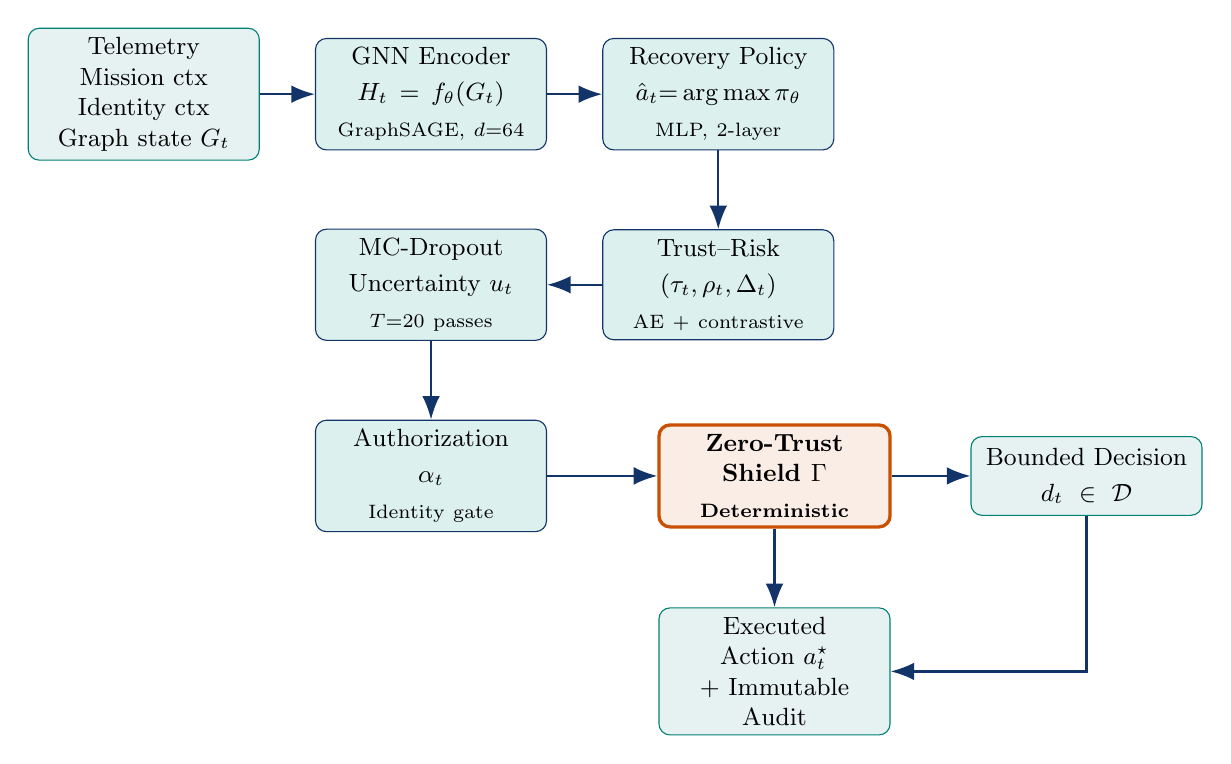
\begin{tikzpicture}[
      node distance=1.0cm and 0.7cm,
      block/.style={draw=navyblue, rounded corners=4pt, align=center,
                    minimum height=1.0cm, minimum width=2.8cm,
                    fill=lightteal, text width=2.7cm, font=\small},
      io/.style={draw=tealgreen, rounded corners=4pt, align=center,
                 minimum height=1.0cm, minimum width=2.8cm,
                 fill=tealgreen!10, text width=2.7cm, font=\small},
      snode/.style={draw=alertorange, very thick, rounded corners=4pt, align=center,
                     minimum height=1.0cm, minimum width=2.8cm,
                     fill=alertorange!10, text width=2.7cm, font=\small\bfseries},
      arr/.style={-{Latex[length=3mm]}, thick, color=navyblue}
  ]
  %% ---- Row 1 (top, left→right): Observation → Encoding → Policy
  \node[io]                         (input)  {Telemetry\\Mission ctx\\Identity ctx\\Graph state $G_t$};
  \node[block, right=of input]      (enc)    {GNN Encoder\\[2pt]$H_t = f_\theta(G_t)$\\[2pt]\scriptsize GraphSAGE, $d{=}64$};
  \node[block, right=of enc]        (policy) {Recovery Policy\\[2pt]$\hat{a}_t{=}\arg\max\pi_\theta$\\[2pt]\scriptsize MLP, 2-layer};

  %% ---- Row 2 (middle, right→left): Trust-Risk ← MC-Dropout
  %%  placed directly below policy (right end) going left
  \node[block, below=1.0cm of policy] (tr)   {Trust--Risk\\[2pt]$(\tau_t,\rho_t,\Delta_t)$\\[2pt]\scriptsize AE + contrastive};
  \node[block, left=of tr]            (unc)  {MC-Dropout\\[2pt]Uncertainty $u_t$\\[2pt]\scriptsize $T{=}20$ passes};

  %% ---- Row 3 (lower, left→right): Auth → Shield → Outcome
  %%  authz is placed below unc so the arrow unc→authz is a clean vertical
  \node[block, below=1.0cm of unc]    (authz)   {Authorization\\[2pt]$\alpha_t$\\[2pt]\scriptsize Identity gate};
  \node[snode, right=1.4cm of authz]  (shield)  {Zero-Trust\\Shield $\Gamma$\\[2pt]\scriptsize Deterministic};
  \node[io,    right=1.0cm of shield] (outcome) {Bounded Decision\\[2pt]$d_t \in \mathcal{D}$};

  %% ---- Row 4 (bottom): Execution below shield
  \node[io, below=1.0cm of shield]    (exec)    {Executed Action $a_t^\star$\\+ Immutable Audit};

  %% ---- Arrows (zero crossing by construction)
  \draw[arr] (input)  -- (enc);
  \draw[arr] (enc)    -- (policy);
  \draw[arr] (policy) -- (tr);      %% vertical down
  \draw[arr] (tr)     -- (unc);     %% horizontal left (same row)
  \draw[arr] (unc)    -- (authz);   %% vertical down
  \draw[arr] (authz)  -- (shield);  %% horizontal right (same row)
  \draw[arr] (shield) -- (outcome); %% horizontal right
  \draw[arr] (shield) -- (exec);    %% vertical down
  \draw[arr] (outcome.south) |- (exec.east); %% elbow: down then left to exec right side
  \end{tikzpicture}%
  }
  \end{center}
  \vspace{0.05cm}
  \begin{center}
    \small\textit{Design principle:} \textbf{The policy proposes; the shield decides admissibility.}
    \quad AI-native coverage $\eta_\text{AI} = 5/6$.
  \end{center}
\end{frame}

\begin{frame}[t,shrink=25]{Architecture}{Five-Layer Component Breakdown}
  \vspace{0.1cm}
  \footnotesize
  \renewcommand{\arraystretch}{1.3}
  \centering
  \begin{tabular}{p{0.25cm}p{2.4cm}p{2.9cm}p{3.4cm}p{2.0cm}}
    \toprule
    \# & \textbf{Component} & \textbf{Architecture} & \textbf{Role} & \textbf{Parameters} \\
    \midrule
    1 & GNN Encoder $f_\theta$ \newline {\color{tealgreen}\textit{(learned)}} & 2-layer GraphSAGE \cite{hamilton2017graphsage}, mean aggregation, $d{=}64$, ReLU & Encodes graph topology into node and graph-level embeddings & ${\approx}4.5$K \\
    \midrule
    2 & Recovery Policy $\pi_\theta$ \newline {\color{tealgreen}\textit{(learned)}} & 2-layer MLP: $[h_a \| \bar{h}_{G_t}] \to$ action logits, softmax & Proposes the best candidate recovery action $\hat{a}_t$ & ${\approx}8.5$K \\
    \midrule
    3 & Trust--Risk Evaluator $Q_\phi$ \newline {\color{tealgreen}\textit{(learned)}} & Autoencoder (trust $\tau_t$) + Contrastive encoder (divergence $\Delta_t$) + Neural risk scorer ($\rho_t$) & Dual-hypothesis safety assessment under benign vs.\ adversarial hypothesis & ${\approx}6.9$K \\
    \midrule
    4 & MC-Dropout $U_\omega$ \newline {\color{tealgreen}\textit{(learned)}} & $T{=}20$ stochastic forward passes; variance over action distribution & Epistemic uncertainty estimation \cite{gal2016dropout}; triggers escalation or block when $u_t$ is high & $p{=}0.1$ \\
    \midrule
    5 & Zero-Trust Shield $\Gamma$ \newline {\color{alertorange}\textit{(deterministic)}} & 14 calibrated scalar thresholds; formal admissibility gate (Algorithm 1) & Sole decision authority; enforces all 5 outcomes; formally verified \cite{rose2020nist} & 14 scalars \\
    \midrule
      & \textbf{Total} & & & $\approx\mathbf{20}$K + shield \\
    \bottomrule
  \end{tabular}
  \vspace{0.15cm}
  {\scriptsize
  \textbf{Notation:}\quad
  $f_\theta$: GNN encoder;\quad $\pi_\theta$: recovery policy;\quad $Q_\phi$: trust–risk evaluator;\quad
  $\tau_t$: trust score;\quad $\rho_t$: risk score;\quad $\Delta_t$: hypothesis divergence;\quad
  $U_\omega$: MC-Dropout uncertainty module;\quad $u_t$: epistemic uncertainty;\quad
  $\Gamma$: zero-trust shield;\quad $d_t$: shield decision;\quad $d$: embedding dim.;\quad $p$: dropout rate.\quad
  Model memory ${\le}2$\,MB — edge-deployable, no GPU at inference.
  }
\end{frame}

% ============================================================
%  SECTION 7 — METHODOLOGY
% ============================================================
\begin{frame}[t,shrink=20]{Methodology}{Zero-Trust Shield Algorithm}
  \begin{columns}[t]
    \column{0.52\textwidth}
    \vspace{0.1cm}
    \begin{block}{Shield Decision Logic (Algorithm 1)}
      \footnotesize
      \begin{enumerate}\tightlist
        \item Encode: $H_t \gets f_\theta(G_t)$
        \item Policy: $\hat{a}_t \gets \arg\max\,\pi_\theta(a|s_t)$
        \item Authorization: $\alpha_t \gets A(i_t, \hat{a}_t, s_t)$
        \item Trust: $\tau_t \gets T_\phi(s_t)$ \quad (AE recon.\ error)
        \item Risk: $\rho_t \gets R_\phi(\hat{a}_t, s_t)$
        \item Divergence: $\Delta_t = \|q_\phi^{(0)} - q_\phi^{(1)}\|_2$
        \item Uncertainty: $u_t \gets U_\omega(s_t, \hat{a}_t)$
        \item Conservatism: $g_t = w_1(1{-}\tau_t)+w_2\rho_t+w_3 u_t+w_4\Delta_t$
      \end{enumerate}
    \end{block}
    \vspace{0.2cm}
    \begin{alertblock}{Graduated Output Rule}
      \footnotesize
      \begin{itemize}\tightlist
        \item $\alpha_t{=}0$ or $\Delta_t{>}\delta^\text{hard}_\text{max}$ $\Rightarrow$ \textbf{block}
        \item $g_t{<}\gamma_1$ and $\tau_t{\ge}\tau_\text{min}$ $\Rightarrow$ \textbf{allow}
        \item $\gamma_1{\le}g_t{<}\gamma_2$ $\Rightarrow$ \textbf{scope-reduce}
        \item $\gamma_2{\le}g_t{<}\gamma_3$ $\Rightarrow$ \textbf{defer}
        \item $\gamma_3{\le}g_t{<}\gamma_4$ or $u_t{>}u_\text{max}$ $\Rightarrow$ \textbf{escalate}
        \item else $\Rightarrow$ \textbf{block}
      \end{itemize}
    \end{alertblock}
    \column{0.44\textwidth}
    \begin{block}{Training Pipeline}
      \footnotesize
      \begin{itemize}\tightlist
        \item 2,000 simulated episodes; ${\approx}60$K annotated steps
        \item 70/15/15 train/val/test split
        \item All 4 attack conditions + clean
      \end{itemize}
      \vspace{0.15cm}
      \renewcommand{\arraystretch}{1.1}
      \begin{tabular}{@{}lcc@{}}
        \toprule
        \textbf{Component} & \textbf{Loss} & \textbf{Epochs} \\
        \midrule
        GNN + Policy & CE & 15--20 \\
        Trust AE & MSE & 10--20 \\
        Risk scorer & BCE & 25--30 \\
        Contrastive enc. & Margin & 40--50 \\
        Shield $\Gamma$ & Calibration & --- \\
        \bottomrule
      \end{tabular}
    \end{block}
    \vspace{0.2cm}
    \begin{exampleblock}{Complexity}
      \footnotesize Per-decision: $\mathcal{O}(L|E_t|d + |\mathcal{A}|k)$\\
      Threshold calibration: $\mathcal{O}_P(1/\sqrt{n})$ convergence
    \end{exampleblock}
  \end{columns}
\end{frame}

\begin{frame}[t,shrink=12]{Methodology}{10 Formal Theoretical Properties}
  \begin{columns}[t]
    \column{0.48\textwidth}
    \begin{block}{Safety Properties}
      \footnotesize
      \begin{enumerate}\tightlist
        \item[\textbf{P1}] \textbf{Monotone conservatism:} worsening any signal ($\uparrow\rho_t$, $\downarrow\tau_t$, $\uparrow u_t$, $\uparrow\Delta_t$) cannot produce a less conservative decision \cite{alshiekh2018shielding}
        \item[\textbf{P2}] \textbf{Unauthorized-actuation exclusion:} $\alpha_t{=}0 \Rightarrow d_t{=}\textsc{block}$ (always)
        \item[\textbf{P3}] \textbf{Divergence safeguard:} $\Delta_t{>}\delta^\text{hard}_\text{max} \Rightarrow d_t{=}\textsc{block}$
        \item[\textbf{P4}] \textbf{Bounded completeness:} $\Gamma$ is a total function — every input maps to exactly one $d_t \in \mathcal{D}$
        \item[\textbf{P5}] \textbf{Complexity bound:} $\mathcal{O}(L|E_t|d + |\mathcal{A}|k)$
        \item[\textbf{P6}] \textbf{Defense-in-depth:} $\Pr[\textsc{allow}|\text{attack}] \le \varepsilon_\alpha \cdot \varepsilon_\tau$ (independent gates multiply)
      \end{enumerate}
    \end{block}
    \column{0.48\textwidth}
    \begin{block}{Statistical \& Utility Properties}
      \footnotesize
      \begin{enumerate}\tightlist
        \item[\textbf{P7}] \textbf{Calibration accuracy:} $\Pr[\varepsilon^\star \le \hat\varepsilon + \sqrt{\ln(1/\delta)/(2n)}] \ge 1-\delta$ (Hoeffding) \cite{angelopoulos2023conformal}
        \item[\textbf{P8}] \textbf{Bounded price of safety:} $\mathbb{E}[\text{utility loss}] \le \eta \cdot U_\text{gap} + \eta_\text{block} \cdot U_\text{max}$
        \item[\textbf{P9}] \textbf{Conformal coverage:} distribution-free guarantee that unsafe actions are blocked with probability ${\ge}1{-}\alpha$ \cite{angelopoulos2023conformal}
        \item[\textbf{P10}] \textbf{Calibration convergence:} $|\gamma_1^{(n)} - \gamma_1^\star| = \mathcal{O}_P(1/\sqrt{n})$
      \end{enumerate}
    \end{block}
    \vspace{0.15cm}
    \begin{alertblock}{Key Insight}
      \footnotesize The deterministic shield is \textbf{policy-agnostic}: any future controller (RL agent, LLM-based planner \cite{toward_autonomous_oran_2026}) can serve as proposal generator without modifying the shield.
    \end{alertblock}
  \end{columns}
\end{frame}

% ============================================================
%  SECTION 8 — RESULTS
% ============================================================
\begin{frame}[t,shrink=12]{Results}{RQ1 --- Security Effectiveness Under Attack}
  \begin{columns}[t]
    \column{0.52\textwidth}
    \begin{center}
      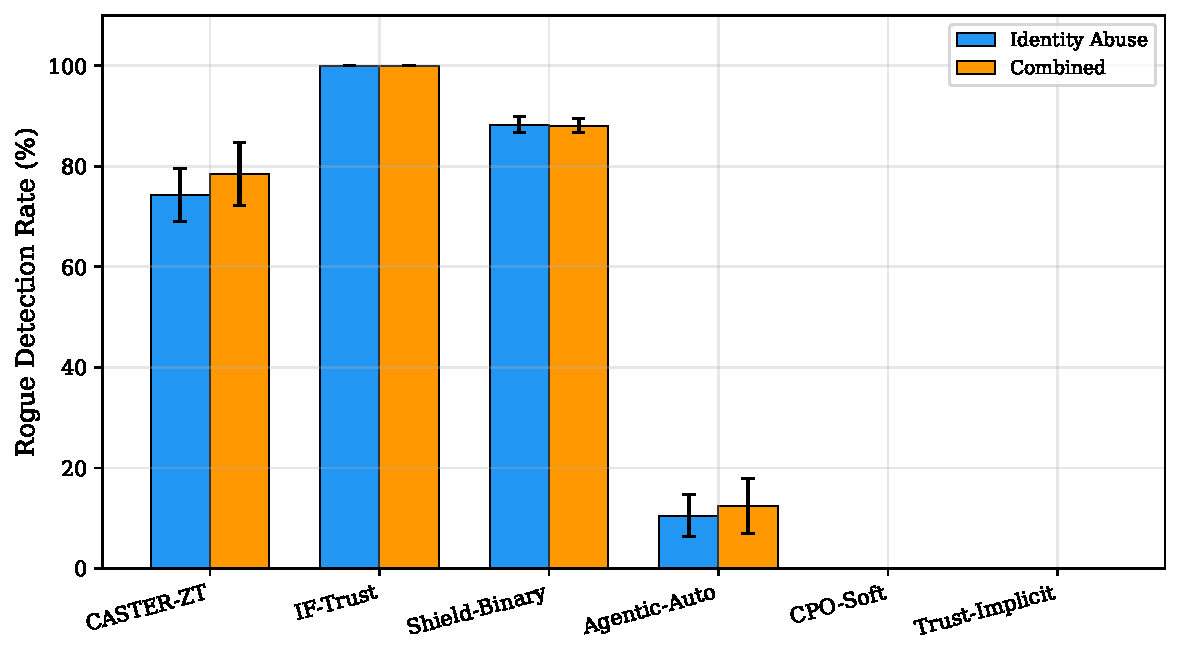
\includegraphics[width=\linewidth,keepaspectratio]{fig_rogue_detection.pdf}
    \end{center}
    \vspace{-0.1cm}
    {\tiny\textit{Rogue detection and blocking under high-severity identity abuse. CASTER-ZT: 74.2\% detection, \textbf{zero false positives}; Shield-Binary: 88.3\% with 48.8\% FP.}}
    \column{0.44\textwidth}
    \begin{block}{Key Results — High-Severity Identity Abuse (20 seeds)}
      \footnotesize
      \renewcommand{\arraystretch}{1.15}
      \begin{tabular}{@{}lccc@{}}
        \toprule
        \textbf{Method} & \textbf{RogueDet} & \textbf{FalseBlk} & $\omega_\text{rec}$ \\
        \midrule
        \textbf{CASTER-ZT} & \textbf{.742} & \textbf{.000} & \textbf{.733} \\
        IF-Trust \cite{zahoor2025ifocsvm} & 1.000 & .000 & .925 \\
        Shield-Bin. \cite{alshiekh2018shielding} & .883 & .488 & .758 \\
        Agentic \cite{toward_autonomous_oran_2026} & .105 & .568 & .144 \\
        CPO-Soft \cite{achiam2017cpo} & .000 & .000 & .201 \\
        \bottomrule
      \end{tabular}
    \end{block}
    \vspace{0.15cm}
    \begin{alertblock}{Differentiator}
      \footnotesize \textbf{CASTER-ZT is the only method achieving zero false positives.}
      IF-Trust achieves 100\% detection but throttles ALL actions — even under clean conditions (pathological).
      Shield-Binary blocks 48.8\% of legitimate actions.
    \end{alertblock}
  \end{columns}
\end{frame}

\begin{frame}[t,shrink=18]{Results}{RQ2 — Recovery Quality \& Ablation}
  \begin{columns}[t]
    \column{0.50\textwidth}
    \begin{block}{Recovery Quality — High-Severity Identity Abuse}
      \footnotesize
      \renewcommand{\arraystretch}{1.2}
      \begin{tabular}{@{}lcc@{}}
        \toprule
        \textbf{Method} & $\omega_\text{rec}$ & $p$-value \\
        \midrule
        \textbf{CASTER-ZT} & $\mathbf{0.733 \pm 0.038}$ & --- \\
        IF-Trust & $0.925 \pm 0.000$ & ${<}0.001$ \\
        Shield-Binary & $0.758 \pm 0.013$ & $0.064$ \\
        Agentic-Auto & $0.144 \pm 0.027$ & ${<}0.001$ \\
        CPO-Soft & $0.201 \pm 0.030$ & ${<}0.001$ \\
        Trust-Implicit & $0.201 \pm 0.030$ & ${<}0.001$ \\
        \bottomrule
      \end{tabular}
    \end{block}
    \vspace{0.2cm}
    {\footnotesize Non-shielding baselines achieve only 0.14–0.20 recovery quality ($p{<}0.001$).}
    \column{0.46\textwidth}
    \begin{alertblock}{Ablation Study — What Each Gate Contributes}
      \footnotesize
      \renewcommand{\arraystretch}{1.2}
      \begin{tabular}{@{}lcc@{}}
        \toprule
        \textbf{Ablation} & \textbf{RogueDet} & $\omega_\text{rec}$ \\
        \midrule
        \textbf{Full CASTER-ZT} & \textbf{.742} & \textbf{.733} \\
        $-$Trust & .524 & .380 \\
        $-$Risk & .665 & .678 \\
        $-$Authorization & .763 & .760 \\
        \bottomrule
      \end{tabular}
    \end{alertblock}
    \vspace{0.2cm}
    \begin{exampleblock}{Finding}
      \footnotesize \textbf{Trust assessment is the critical gate:} removing it causes RogueDet to drop from 0.742 to 0.524 and $\omega_\text{rec}$ from 0.733 to 0.380 ($p{<}0.001$).\\
      \textbf{Validates Proposition~6}: independent gates multiply to reduce unsafe execution probability.
    \end{exampleblock}
  \end{columns}
\end{frame}

\begin{frame}[t,shrink=14]{Results}{RQ3 --- Generalization Across Scales \& Severities}
  \begin{columns}[t]
    \column{0.52\textwidth}
    \begin{center}
      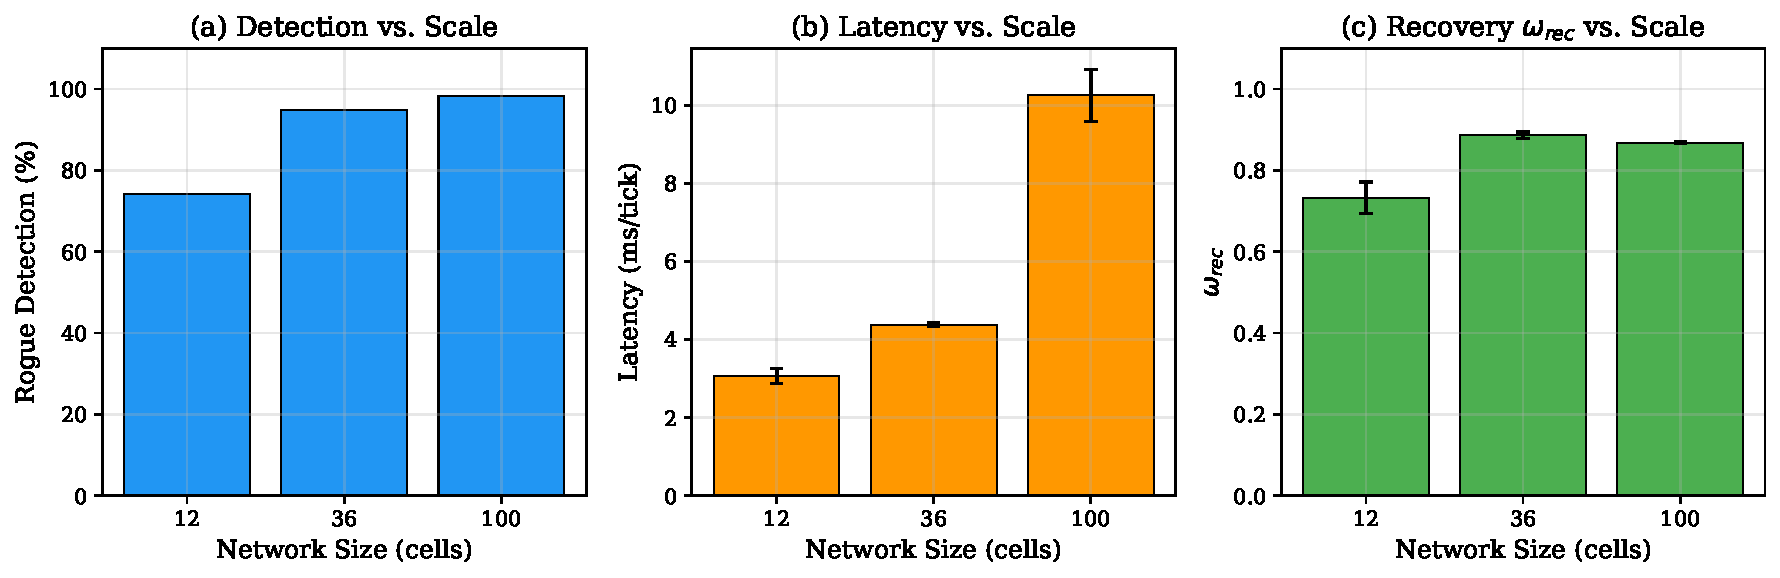
\includegraphics[width=\linewidth,keepaspectratio]{fig_multiscale.pdf}
    \end{center}
    \vspace{-0.1cm}
    {\tiny\textit{Security improves with scale; 12-cell latency is $3\times$ below O-RAN 10\,ms budget.}}
    \column{0.44\textwidth}
    \begin{block}{Multi-Scale Results — High-Severity Identity Abuse}
      \footnotesize
      \renewcommand{\arraystretch}{1.2}
      \begin{tabular}{@{}lccc@{}}
        \toprule
        \textbf{Topology} & \textbf{RogueDet} & $\omega_\text{rec}$ & \textbf{Latency} \\
        \midrule
        12-cell, 2-zone & 0.742 & 0.733 & 3.07\,ms \\
        36-cell, 4-zone & 0.949 & 0.886 & 4.38\,ms \\
        100-cell, 8-zone & 0.983 & 0.868 & 10.25\,ms \\
        \bottomrule
      \end{tabular}
    \end{block}
    \vspace{0.2cm}
    \begin{exampleblock}{Key Observations}
      \footnotesize
      \begin{itemize}\tightlist
        \item Detection \textbf{improves with scale} (richer structural context for GNN)
        \item Latency scales \textbf{within O-RAN budget} at 12 and 36 cells
        \item Zero false positives \textbf{across all scales} and all $\gamma_1 \in \{0.10,\ldots,0.60\}$ (threshold sensitivity confirmed)
        \item Severity: RogueDet 0.806 (medium) $\to$ 0.742 (high) — consistent degradation
      \end{itemize}
    \end{exampleblock}
  \end{columns}
\end{frame}

\begin{frame}[t,shrink=10]{Results}{RQ4 — 6G Deployment Compliance}
  \begin{columns}[t]
    \column{0.36\textwidth}
    \vspace{0.1cm}
    \begin{block}{Deployment Profile}
      \scriptsize
      \renewcommand{\arraystretch}{1.2}
      \begin{tabular}{@{}lcc@{}}
        \toprule
        \textbf{Metric} & \textbf{Value} & \textbf{Limit} \\
        \midrule
        Latency (12-cell) & 3.07\,ms & ${<}10$ \cmark \\
        Latency (36-cell) & 4.38\,ms & ${<}10$ \cmark \\
        Latency (100-cell) & 10.25\,ms & ${<}10$ \pmark \\
        Model memory & ${\le}2$\,MB & ${<}50$ \cmark \\
        Parameters & $\approx20$K & --- \\
        AI-native $\eta_\text{AI}$ & $5/6$ & --- \cmark \\
        Audit completeness & 100\% & Req.~\cmark \\
        Edge autonomy & Yes & Req.~\cmark \\
        \bottomrule
      \end{tabular}
    \end{block}
    \vspace{0.2cm}
    \begin{alertblock}{\scriptsize 100-cell note}
      \scriptsize 10.25\,ms marginally exceeds O-RAN 10\,ms budget. Future work: quantization, edge batching.
    \end{alertblock}
    \column{0.60\textwidth}
    \begin{center}
      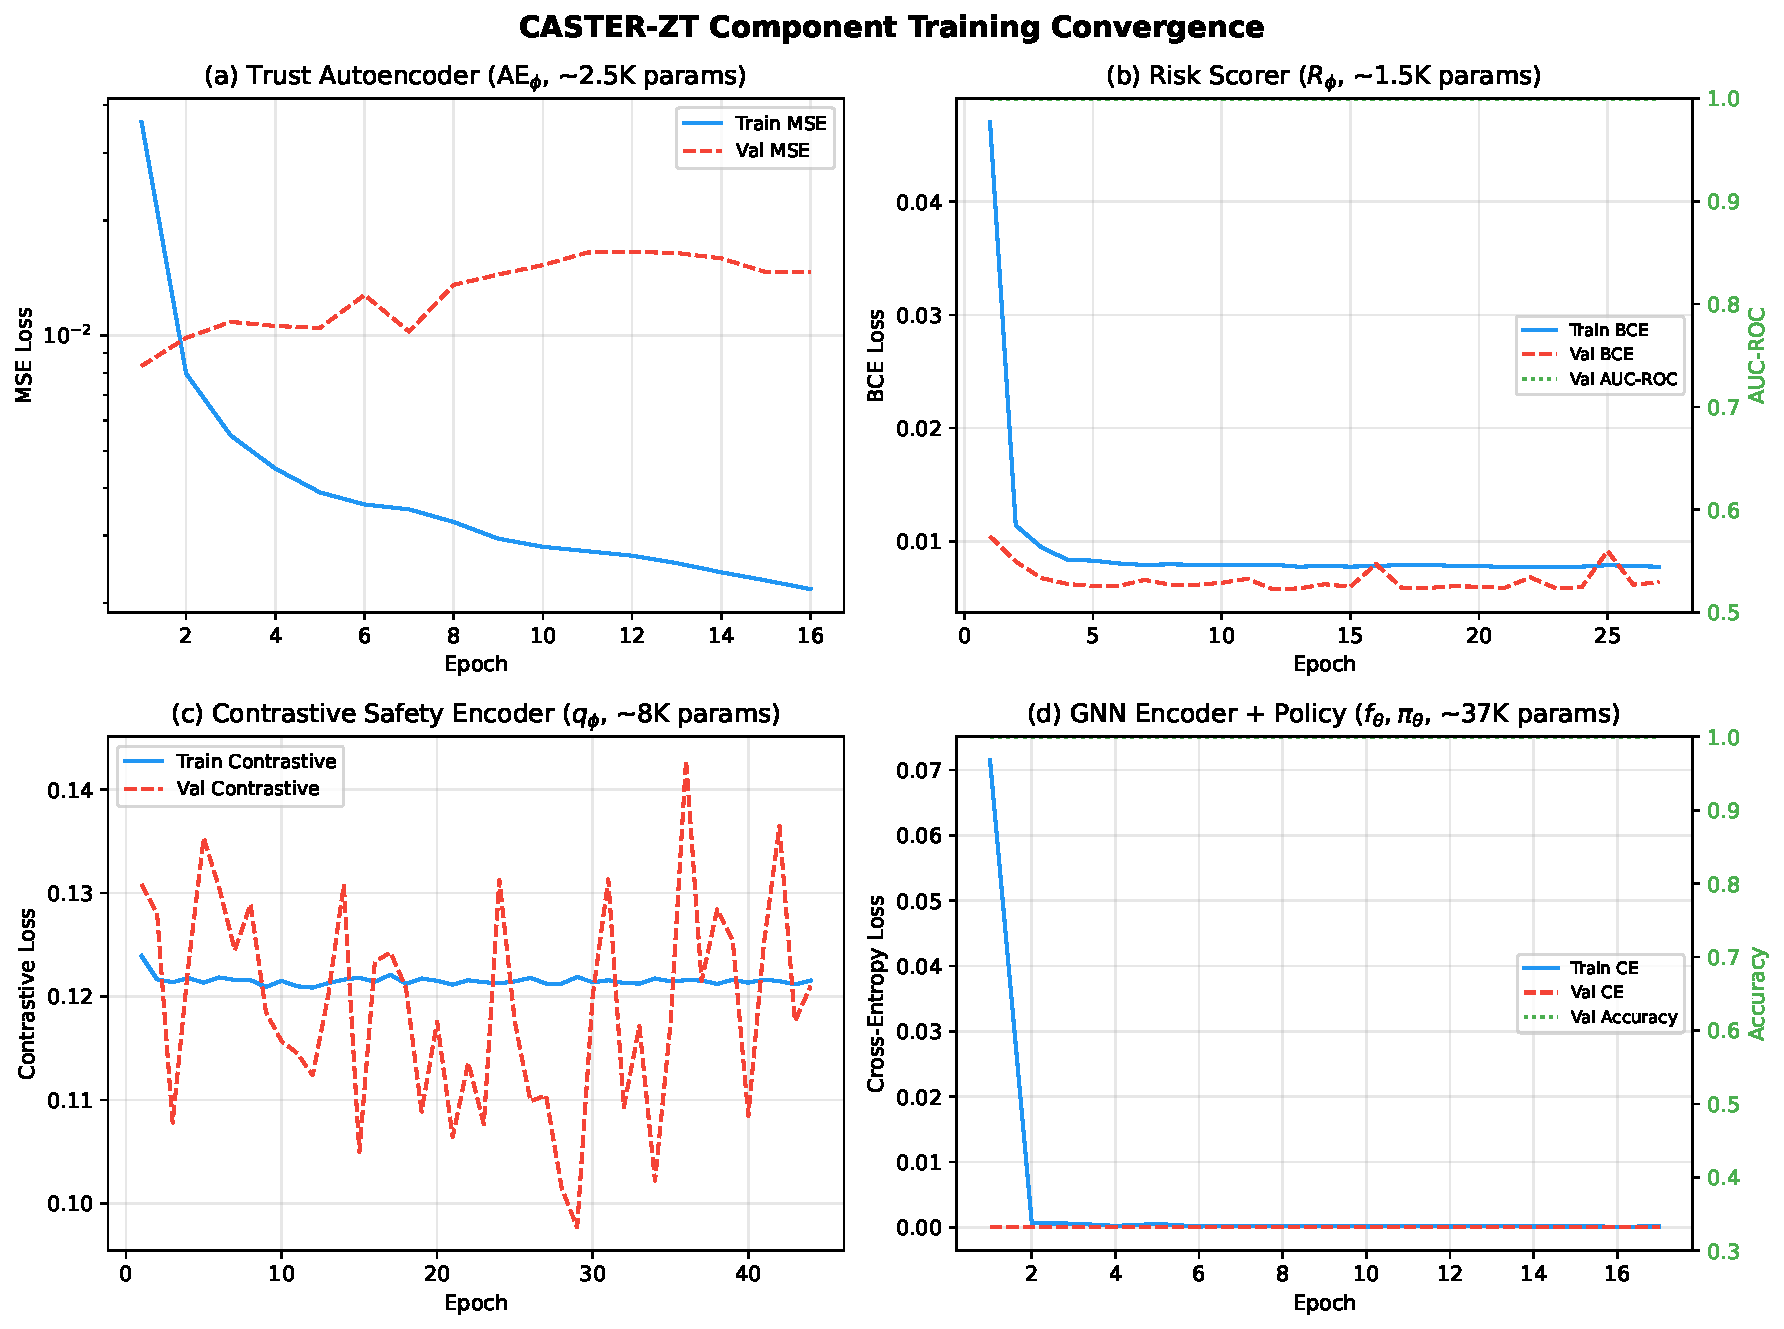
\includegraphics[width=\linewidth,height=0.72\textheight,keepaspectratio]{fig_training_curves.pdf}
    \end{center}
    {\tiny\textit{Training convergence for all 4 learned components ($\approx$20,019 params). Trust AE: MSE by epoch~16. Risk scorer: BCE, AUC$=0.999$ by epoch~27. Contrastive encoder: margin by epoch~44. GNN+Policy: CE, acc$=1.000$ by epoch~17.}}
  \end{columns}
\end{frame}

% ============================================================
%  SECTION 9 — PROGRESS & FUTURE WORK
% ============================================================
\begin{frame}[t,shrink=35]{Progress \& Future Work}{}
  \begin{columns}[t]
    \column{0.48\textwidth}
    \begin{exampleblock}{\cmark\ Completed Work}
      \begin{itemize}\tightlist
        \item \textbf{Framework:} Full CASTER-ZT pipeline designed and implemented (GNN encoder, policy, trust–risk evaluator, MC-Dropout, shield)
        \item \textbf{Theory:} 10 formal propositions proved (supplemental proofs document)
        \item \textbf{Evaluation:} 2,420-run campaign (11 methods $\times$ 7 conditions $\times$ 20 seeds + multi-scale)
        \item \textbf{Baselines:} 4 external baselines + 6 ablations faithfully implemented
        \item \textbf{Data:} 4-layer data provenance (synthetic + 5G real distributions + SWaT/WADI grounding + conformal calibration)
        \item \textbf{Compliance:} 6G near-RT, O-RAN, EU AI Act requirements analyzed and met at primary scale
        \item \textbf{Paper:} Manuscript drafted for IEEE Transactions on Mobile Computing (TMC) — \textit{(Submitted)}
      \end{itemize}
    \end{exampleblock}
    \column{0.48\textwidth}
    \begin{alertblock}{\pmark\ Limitations \& Future Work}
      \begin{itemize}\tightlist
        \item \textbf{Trust AE vs.\ telemetry poisoning:} reconstruction-error detector does not hard-block sophisticated poisoning attacks \cite{pang2021deep,kravchik2022efficient}\\
              $\hookrightarrow$ \textit{Plan: cross-source GNN consistency checking, adversarially trained detectors, temporal sequence modeling}
        \item \textbf{100-cell latency:} 10.25\,ms marginally exceeds O-RAN 10\,ms budget\\
              $\hookrightarrow$ \textit{Plan: model quantization, edge batching, hardware profiling}
        \item \textbf{Policy learning:} current policy trained via supervised imitation\\
              $\hookrightarrow$ \textit{Plan: RL-based online policy optimization under shield constraints}
        \item \textbf{Adaptive adversaries:} adversary cannot currently modify shield internals\\
              $\hookrightarrow$ \textit{Plan: evaluation under adaptive attackers, multi-zone scenarios}
        \item \textbf{Agentic integration:} combine with LLM-based orchestrator as proposal generator \cite{toward_autonomous_oran_2026,lee2024llmran}
      \end{itemize}
    \end{alertblock}
  \end{columns}
\end{frame}

% ============================================================
%  CONCLUSION
% ============================================================
\begin{frame}[t,shrink=12]{Conclusion}{}
  \begin{columns}[t]
    \column{0.55\textwidth}
    \begin{block}{Summary}
      \begin{itemize}\tightlist
        \item Proposed \textbf{CASTER-ZT}: first framework combining graph-structured decision making with formally bounded zero-trust admissibility for disaster-recovery autonomy
        \item \textbf{10 formal properties}: defense-in-depth, conformal coverage, calibration convergence
        \item \textbf{Zero false positives} across all conditions — unique among all evaluated methods
        \item \textbf{3.07\,ms} per-decision latency — within O-RAN Near-RT RIC budget
        \item \textbf{$\approx$20K params, $\le$2\,MB} — fully edge-deployable, no GPU
        \item Policy-agnostic shield: future-proof for RL or LLM-based proposal generators
      \end{itemize}
    \end{block}
    \column{0.40\textwidth}
    \begin{center}
      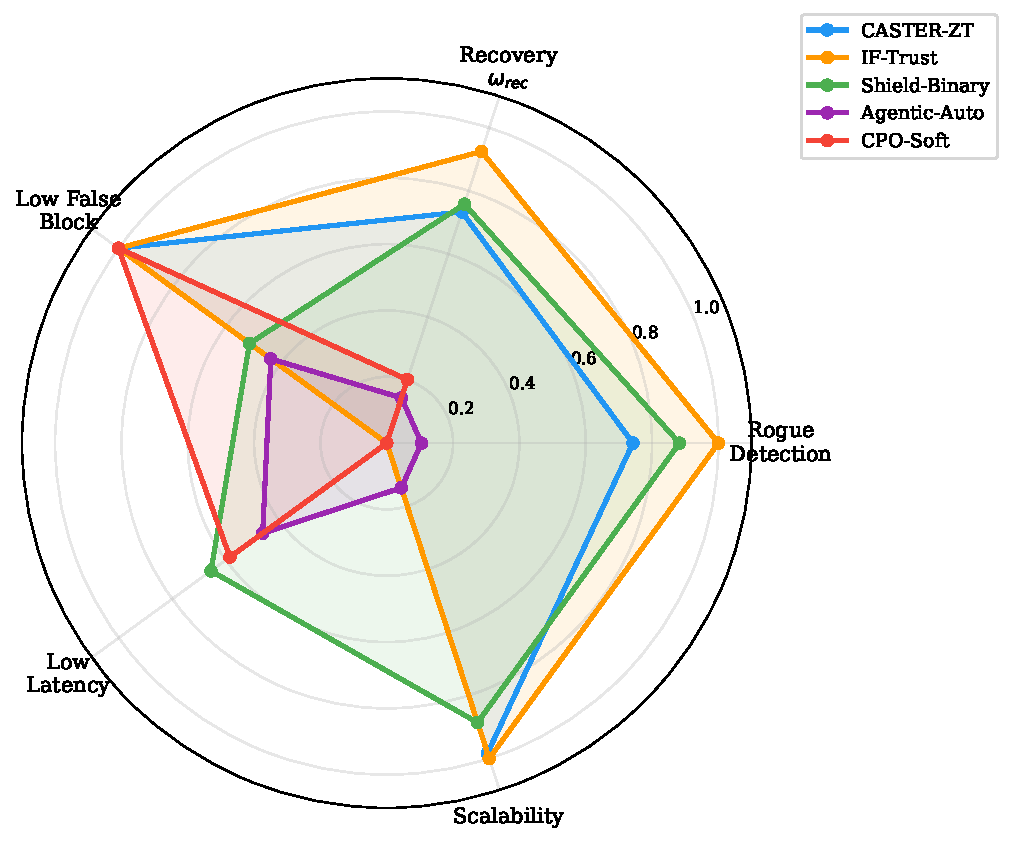
\includegraphics[width=\linewidth,keepaspectratio]{fig_radar_comparison.pdf}
    \end{center}
    {\tiny\textit{Radar: CASTER-ZT unique zero-FP, graduated-enforcement profile under high-severity identity abuse.}}
  \end{columns}
  \vspace{0.3cm}
  \begin{exampleblock}{Bottom Line}
    \centering\small
    \textbf{Security-first $\neq$ utility-last.}\quad
    CASTER-ZT proves you can enforce formal zero-trust boundaries \textit{and} deliver meaningful autonomous recovery.
  \end{exampleblock}
\end{frame}

% ============================================================
%  REFERENCES — Slide 1
% ============================================================
\begin{frame}[allowframebreaks]{References}
  \tiny
  \bibliographystyle{IEEEtran}
  \bibliography{references}
\end{frame}

\end{document}
